\chapter{Structure \& Components of the Framework}
\label{ch:framework}

This chapter details the technical implementation of the \apsq framework and is mostly intended to provide insight into the gearbox to potential developers and interested users.
The framework consists of the following four main components that together form \apsq:
\begin{enumerate}
\item \textbf{Core}: The core contains the internal logic to initialize the modules, provide the geometry, facilitate module communication and run the event sequence.
The core keeps its dependencies to a minimum (it only relies on ROOT) and remains independent from the other components as far as possible.
It is the main component discussed in this section.
\item \textbf{Modules}: A module is a set of methods which is executed as part of the simulation chain.
Modules are built as separate libraries and loaded dynamically on demand by the core.
The available modules and their parameters are discussed in detail in Chapter~\ref{ch:modules}.
\item \textbf{Objects}: Objects form the data passed between modules using the message framework provided by the core.
Modules can listen and bind to messages with objects they wish to receive.
Messages are identified by the object type they are carrying, but can also be renamed to allow the direction of data to specific modules, facilitating more sophisticated simulation setups.
Messages are intended to be read-only and a copy of the data should be made if a module wishes to change the data.
All objects are compiled into a separate library which is automatically linked to every module.
More information about the messaging system and the supported objects can be found in Section~\ref{sec:objects_messages}.
\item \textbf{Physics}: In many cases, several modules depend on the same underlying physics models.
These models are separated by the modules themselves.
The implemented physics models are described in Chapter~\ref{ch:models}.
\item \textbf{Tools}: \apsq provides a set of header-only 'tools' and a shared library that allow access to common logic shared by various modules.
Examples are the Runge-Kutta solver~\cite{fehlberg} implemented using the Eigen3 library and the set of template specializations for ROOT and Geant4 configurations.
More information about the tools can be found in Chapter~\ref{ch:additional_tools_resources}.
This set of tools is different from the set of core utilities the framework itself provides, which is part of the core and explained in Section~\ref{sec:logging_utilities}.
\end{enumerate}
Finally, \apsq provides an executable which instantiates the core of the framework, receives and distributes the configuration object and runs the simulation chain.

The chapter is structured as follows.
Section~\ref{sec:arch} provides an overview of the architectural design of the core and describes its interaction with the rest of the \apsq framework.
The different subcomponents such as configuration, modules and messages are discussed in Sections~\ref{sec:config_parameters}--\ref{sec:objects_messages}.
The chapter closes with a description of the available framework tools in Section~\ref{sec:logging_utilities}.
Some \CPP code will be provided in the text, but readers not interested may skip the technical details.

\section{Architecture of the Core}
\label{sec:arch}
The core is constructed as a light-weight framework which provides various subsystems to the modules.
It contains the part of the software responsible for instantiating and running the modules from the supplied configuration file, and is structured around five subsystems, of which four are centered around a manager and the fifth contains a set of general utilities.
The systems provided are:
\begin{enumerate}
\item \textbf{Configuration}: The configuration subsystem provides a configuration object from which data can be retrieved or stored, together with a TOML-like~\cite{tomlgit} parser to read configuration files.
It also contains the \apsq configuration manager which provides access to the main configuration file and its sections.
It is used by the module manager system to find the required instantiations and access the global configuration.
More information is given in Section~\ref{sec:config_parameters}.
\item \textbf{Module}: The module subsystem contains the base class of all \apsq modules as well as the manager responsible for loading and executing the modules (using the configuration system).
This component is discussed in more detail in Section~\ref{sec:module_manager}.
\item \textbf{Geometry}: The geometry subsystem supplies helpers for the simulation geometry.
The manager instantiates all detectors from the detector configuration file.
A detector object contains the position and orientation linked to an instantiation of a particular detector model, itself containing all parameters describing the geometry of the detector.
More details about geometry and detector models is provided in Section~\ref{sec:models_geometry}.
\item \textbf{Messenger}: The messenger is responsible for sending objects from one module to another.
The messenger object is passed to every module and can be used to bind to messages to listen for.
Messages with objects are also dispatched through the messenger as described in Section~\ref{sec:objects_messages}.
\item \textbf{Utilities}: The framework provides a set of utilities for logging, file and directory access, and unit conversion.
An explanation on how to use of these utilities can be found in Section~\ref{sec:logging_utilities}.
A set of \CPP exceptions is also provided in the utilities, which are inherited and extended by the other components.
Proper use of exceptions, together with logging information and reporting errors, makes the framework easier to use and debug.
A few notes about the use and structure of exceptions are provided in Section~\ref{sec:error_reporting_exceptions}.
\end{enumerate}

\section{Configuration and Parameters}
\label{sec:config_parameters}
Individual modules as well as the framework itself are configured through configuration files, which all follow the same format.
Explanations on how to use the various configuration files together with several examples have been provided in Section~\ref{sec:configuration_files}.

\subsection{File format}
\label{sec:config_file_format}
Throughout the framework, a simplified version of TOML~\cite{tomlgit} is used as standard format for configuration files.
The format is defined as follows:
\begin{enumerate}
\item All whitespace at the beginning or end of a line are stripped by the parser.
In the rest of this format specification the \textit{line} refers to the line with this whitespace stripped.
\item Empty lines are ignored.
\item Every non-empty line should start with either \texttt{\#}, \texttt{[} or an alphanumeric character.
Every other character should lead to an immediate parse error.
\item If the line starts with a hash character (\texttt{\#}), it is interpreted as comment and all other content on the same line is ignored.
\item If the line starts with an open square bracket (\texttt{[}), it indicates a section header (also known as configuration header).
The line should contain a string with alphanumeric characters and underscores, indicating the header name, followed by a closing square bracket (\texttt{]}), to end the header.
After any number of ignored whitespace characters there could be a \texttt{\#} character.
If this is the case, the rest of the line is handled as specified in point~3.
Otherwise there should not be any other character (except the whitespace) on the line.
Any line that does not comply to these specifications should lead to an immediate parse error.
Multiple section headers with the same name are allowed.
All key-value pairs following this section header are part of this section until a new section header is started.
\item If the line starts with an alphanumeric character, the line should indicate a key-value pair.
The beginning of the line should contain a string of alphabetic characters, numbers, dots (\texttt{.}), colons (\texttt{\:}) and underscores (\texttt{\_}), but it may only start with an alphanumeric character.
This string indicates the 'key'.
After an optional number of ignored whitespace, the key should be followed by an equality sign (\texttt{$=$}).
Any text between the \texttt{$=$} and the first \texttt{\#} character not enclosed within a pair of single or double quotes (\texttt{'} or \texttt{"}) is known as the non-stripped string.
Any character after the \texttt{\#} is handled as specified in point 3.
If the line does not contain any non-enclosed \texttt{\#} character, the value ends at the end of the line instead.
The 'value' of the key-value pair is the non-stripped string with all whitespace in front and at the end stripped.
The value may not be empty.
Any line that does not comply to these specifications should lead to an immediate parse error.
\item The value may consist of multiple nested dimensions which are grouped by pairs of square brackets (\texttt{[} and \texttt{]}).
The number of square brackets should be properly balanced, otherwise an error is raised.
Square brackets which should not be used for grouping should be enclosed in quotation marks.
Every dimension is split at every whitespace sequence and comma character (\texttt{,}) not enclosed in quotation marks.
Implicit square brackets are added to the begin and end of the value, if these are not explicitly added.
A few situations require explicit addition of outer brackets such as matrices with only one column element, i.e. with dimension 1xN.
\item The sections of the value which are interpreted as separate entities are named elements.
For a single value the element is on the zeroth dimension, for arrays on the first dimension and for matrices on the second dimension.
Elements can be forced by using quotation marks, either single or double quotes (\texttt{'} or \texttt{"}).
The number of both types of quotation marks should be properly balanced, otherwise an error is raised.
The conversion to the elements to the actual type is performed when accessing the value.
\item All key-value pairs defined before the first section header are part of a zero-length empty section header.
\end{enumerate}

\subsection{Accessing parameters}
\label{sec:accessing_parameters}
Values are accessed via the configuration object.
In the following example, the key is a string called \parameter{key}, the object is named \parameter{config} and the type \parameter{TYPE} is a valid \CPP type the value should represent.
The values can be accessed via the following methods:
\begin{minted}[frame=single,framesep=3pt,breaklines=true,tabsize=2,linenos]{c++}
// Returns true if the key exists and false otherwise
config.has("key")
// Returns the number of keys found from the provided initializer list:
config.count({"key1", "key2", "key3"});
// Returns the value in the given type, throws an exception if not existing or a conversion to TYPE is not possible
config.get<TYPE>("key")
// Returns the value in the given type or the provided default value if it does not exist
config.get<TYPE>("key", default_value)
// Returns an array of elements of the given type
config.getArray<TYPE>("key")
// Returns a matrix: an array of arrays of elements of the given type
config.getMatrix<TYPE>("key")
// Returns an absolute (canonical if it should exist) path to a file
config.getPath("key", true /* check if path exists */)
// Return an array of absolute paths
config.getPathArray("key", false /* do not check if paths exists */)
// Returns the value as literal text including possible quotation marks
config.getText("key")
// Set the value of key to the default value if the key is not defined
config.setDefault("key", default_value)
// Set the value of the key to the default array if key is not defined
config.setDefaultArray<TYPE>("key", vector_of_default_values)
// Create an alias named new_key for the already existing old_key or throws an exception if the old_key does not exist
config.setAlias("new_key", "old_key")
\end{minted}

Conversions to the requested type are using the \parameter{from_string} and \parameter{to_string} methods provided by the string utility library described in Section~\ref{sec:string_utilities}.
These conversions largely follow standard \CPP parsing, with one important exception.
If (and only if) the value is retrieved as a C/\CPP string and the string is fully enclosed by a pair of \texttt{"} characters, these are stripped before returning the value.
Strings can thus also be provided with or without quotation marks.

\begin{warning}
    It should be noted that a conversion from string to the requested type is a comparatively heavy operation.
    For performance-critical sections of the code, one should consider fetching the configuration value once and caching it in a local variable.
\end{warning}

\section{Modules and the Module Manager}
\label{sec:module_manager}
\apsq is a modular framework and one of the core ideas is to partition functionality in independent modules which can be inserted or removed as required.
These modules are located in the subdirectory \textit{src/modules/} of the repository, with the name of the directory the unique name of the module.
The suggested naming scheme is CamelCase, thus an example module name would be \textit{GenericPropagation}.
There are two different kind of modules which can be defined:
\begin{itemize}
    \item \textbf{Unique}: Modules for which a single instance runs, irrespective of the number of detectors.
    \item \textbf{Detector}: Modules which are concerned with only a single detector at a time.
    These are then replicated for all required detectors.
\end{itemize}
The type of module determines the constructor used, the internal unique name and the supported configuration parameters.
For more details about the instantiation logic for the different types of modules, see Section~\ref{sec:module_instantiation}.

\subsection{Module instantiation}
\label{sec:module_instantiation}
Modules are dynamically loaded and instantiated by the Module Manager.
They are constructed, initialized, executed and finalized in the linear order in which they are defined in the configuration file; for this reason the configuration file should follow the order of the real process.
For each section in the main configuration file (see~\ref{sec:config_parameters} for more details), a corresponding library is searched for which contains the module (the exception being the global framework section).
Module libraries are always named following the scheme \textbf{libAllpixModule\texttt{ModuleName}}, reflecting the \texttt{ModuleName} configured via CMake.
The module search order is as follows:
\begin{enumerate}
\item Modules already loaded before from an earlier section header
\item All directories in the global configuration parameter \parameter{library_directories} in the provided order, if this parameter exists.
\item The internal library paths of the executable, that should automatically point to the libraries that are built and installed together with the executable.
These library paths are stored in \dir{RPATH} on Linux, see the next point for more information.
\item The other standard locations to search for libraries depending on the operating system.
Details about the procedure Linux follows can be found in~\cite{linuxld}.
\end{enumerate}

If the loading of the module library is successful, the module is checked to determine if it is a unique or detector module.
As a single module may be called multiple times in the configuration, with overlapping requirements (such as a module which runs on all detectors of a given type, followed by the same module but with different parameters for one specific detector, also of this type) the Module Manager must establish which instantiations to keep and which to discard.
The instantiation logic determines a unique name and priority, where a lower number indicates a higher priority, for every instantiation.
The name and priority for the instantiation are determined differently for the two types of modules:
\begin{itemize}
\item \textbf{Unique}: Combination of the name of the module and the \parameter{input} and \parameter{output} parameter (both defaulting to an empty string).
The priority is always zero.
\item \textbf{Detector}: Combination of the name of the module, the \parameter{input} and \parameter{output} parameter (both defaulting to an empty string) and the name of detector this module is executed for.
If the name of the detector is specified directly by the \parameter{name} parameter, the priority is \emph{high}.
If the detector is only matched by the \parameter{type} parameter, the priority is \emph{medium}.
If the \parameter{name} and \parameter{type} are both unspecified and the module is instantiated for all detectors, the priority is \emph{low}.
\end{itemize}
In the end, only a single instance for every unique name is allowed.
If there are multiple instantiations with the same unique name, the instantiation with the highest priority is kept.
If multiple instantiations with the same unique name and the same priority exist, an exception is raised.

\subsection{Multithreading: Parallel execution of events}
\label{sec:multithreading}
The framework supports running several events in parallel via its multithreading feature.
By default, this feature is disabled for new modules.
If supported by all modules in the simulation, multithreading is enabled by default, but can be disabled by the user as described in Section~\ref{sec:framework_parameters}.
When enabled this feature can provide a significant speed improvement, depending on the simulation chain.

The framework allows to parallelize the execution of the same module for multiple events, if these would otherwise be executed directly after each other in a linear order.
Thus, events are added to a work queue and then distributed to a set of worker threads as specified in the configuration or determined from system parameters.

Detailed description of how the framework implements the multithreading feature can be found in Section~\ref{sec:multithreading_approach} and an overview of important considerations when writing a new module capable of multithreading is provided in Section~\ref{sec:module_multithreading}.

\section{Geometry and Detectors}
\label{sec:models_geometry}
Simulations are frequently performed for a set of different detectors (such as a beam telescope and a device under test).
All of these individual detectors together form what \apsq defines as the geometry.
Each detector has a set of properties attached to it:
\begin{itemize}
\item A unique detector \parameter{name} to refer to the detector in the configuration.
\item The \parameter{position} in the world frame.
This is the position of the geometric center of the sensitive device (sensor) given in world coordinates as X, Y and Z as defined in Section~\ref{sec:coordinate_systems} (note that any additional components like the chip and possible support layers are ignored when determining the geometric center).
\item An \parameter{orientation_mode} that determines the way that the orientation is applied.
This can be either \texttt{xyz}, \texttt{zyx} or \texttt{zxz}, where \textbf{\texttt{xyz} is used as default if the parameter is not specified}. Three angles are expected as input, which should always be provided in the order in which they are applied.
\begin{itemize}
    \item The \texttt{xyz} option uses extrinsic Euler angles to apply a rotation around the global $X$ axis, followed by a rotation around the global $Y$ axis and finally a rotation around the global $Z$ axis.
    \item The \texttt{zyx} option uses the \textbf{extrinsic Z-Y-X convention} for Euler angles, also known as Pitch-Roll-Yaw or 321 convention. The rotation is represented by three angles describing first a rotation of an angle $\phi$ (yaw) about the $Z$ axis, followed by a rotation of an angle $\theta$ (pitch) about the initial $Y$ axis, followed by a third rotation of an angle $\psi$ (roll) about the initial $X$ axis.
    \item The \texttt{zxz} uses the \textbf{extrinsic Z-X-Z convention} for Euler angles instead. This option is also known as the 3-1-3 or the "x-convention" and the most widely used definition of Euler angles~\cite{eulerangles}.
\end{itemize}
\begin{warning}
It is highly recommended to always explicitly state the orientation mode instead of relying on the default configuration.
\end{warning}

\item The \parameter{orientation} to specify the Euler angles in logical order (e.g. first $X$, then $Y$, then $Z$ for the \texttt{xyz} method), interpreted using the method above (or with the \texttt{xyz} method if the \parameter{orientation_mode} is not specified). An example for three Euler angles would be
\begin{minted}[frame=single,framesep=3pt,breaklines=true,tabsize=2,linenos]{ini}
orientation_mode = "zyx"
orientation = 45deg 10deg 12deg
\end{minted}
which describes the rotation of \SI{45}{\degree} around the $Z$ axis, followed by a \SI{10}{\degree} rotation around the initial $Y$ axis, and finally a rotation of \SI{12}{\degree} around the initial $X$ axis.
\begin{warning}
All supported rotations are extrinsic active rotations, i.e. the vector itself is rotated, not the coordinate system. All angles in configuration files should be specified in the order they will be applied.
\end{warning}

\item A \parameter{type} parameter describing the detector model, for example \emph{timepix} or \emph{mimosa26}.
These models define the geometry and parameters of the detector.
Multiple detectors can share the same model, several of which are shipped ready-to-use with the framework.
\item An optional parameter \parameter{alignment_precision_position} to specify the alignment precision along the three global axes as described in Section~\ref{sec:detector_config}.
\item An optional parameter \parameter{alignment_precision_orientation} for the alignment precision in the three rotation angles as described in Section~\ref{sec:detector_config}.
\item An optional \textbf{electric field} in the sensitive device.
An electric field can be added to a detector by a special module as demonstrated in Section~\ref{sec:module_electric_field}.
\end{itemize}
The detector configuration is provided in the detector configuration file as explained in Section~\ref{sec:detector_config}.

\subsection{Coordinate systems}
\label{sec:coordinate_systems}

Local coordinate systems for each detector and a global frame of reference for the full setup are defined.
The global coordinate system is chosen as a right-handed Cartesian system, and the rotations of individual devices are performed around the geometrical center of their sensor.

Local coordinate systems for the detectors are also right-handed Cartesian systems, with the x- and y-axes defining the sensor plane.
The origin of this coordinate system is the center of the lower left pixel in the grid, i.e.\ the pixel with indices (0,0).
This simplifies calculations in the local coordinate system as all positions can either be stated in absolute numbers or in fractions of the pixel pitch.

A sketch of the actual coordinate transformations performed, including the order of transformations, is provided in Figure~\ref{fig:transformations}. The global coordinate system used for tracking of particles through detetector setup is shown on the left side, while the local coordinate system used to describe the individual sensors is located at the right.

\begin{figure}[tbp]
  \center
  \input{tikz/transformations}
  \caption{Coordinate transformations from global to local and revers. The first row shows the detector positions in the respective coordinate systems in top view, the second row in side view.}
  \label{fig:transformations}
\end{figure}

The global reference for time measurements is the beginning of the event, i.e.\ the start of the particle tracking through the setup.
The local time reference is the time of entry of the \emph{first} primary particle of the event into the sensor.
This means that secondary particles created within the sensor inherit the local time reference from their parent particles in order to have a uniform time reference in the sensor.
It should be noted that Monte Carlo particles that start the local time frame on different detectors do not necessarily have to belong to the same particle track.

\subsection{Changing and accessing the geometry}
The geometry is needed at a very early stage because it determines the number of detector module instantiations as explained in Section~\ref{sec:module_instantiation}.
The procedure of finding and loading the appropriate detector models is explained in more detail in Section~\ref{sec:detector_models}.

The geometry is directly added from the detector configuration file described in Section~\ref{sec:detector_config}.
The geometry manager parses this file on construction, and the detector models are loaded and linked later during geometry closing as described above.
It is also possible to add additional models and detectors directly using \parameter{addModel} and \parameter{addDetector} (before the geometry is closed).
Furthermore it is possible to add additional points which should be part of the world geometry using \parameter{addPoint}.
This can for example be used to add the beam source to the world geometry.

The detectors and models can be accessed by name and type through the geometry manager using \parameter{getDetector} and \parameter{getModel}, respectively.
All detectors can be fetched at once using the \parameter{getDetectors} method.
If the module is a detector-specific module its related Detector can be accessed through the \parameter{getDetector} method of the module base class instead (returns a null pointer for unique modules) as follows:
\begin{minted}[frame=single,framesep=3pt,breaklines=true,tabsize=2,linenos]{c++}
void run(Event* event) {
    // Returns the linked detector
    std::shared_ptr<Detector> detector = this->getDetector();
}
\end{minted}

\subsection{Detector models}
\label{sec:detector_models}
Different types of detector models are available and distributed together with the framework: these models use the configuration format introduced in Section~\ref{sec:config_file_format} and can be found in the \textit{models} directory of the repository.
Every model extends from the \texttt{DetectorModel} base class, which defines the minimum required parameters of a detector model within the framework.
The coordinates place the detector in the global coordinate system, with the reference point taken as the geometric center of the active matrix.
This is defined by the number of pixels in the sensor in both the x- and y-direction, and together with the pitch of the individual pixels the total size of the pixel matrix is determined.
Outside the active matrix, the sensor can feature excess material in all directions in the x-y-plane.
A detector of base class type does not feature a separate readout chip, thus only the thickness of an additional, inactive silicon layer can be specified.
Derived models allow for separate readout chips, optionally connected with bump bonds.

The base detector model can be extended to provide more detailed geometries.
Currently implemented derived models are the \texttt{MonolithicPixelDetectorModel}, which describes a monolithic detector with all electronics directly implemented in the same silicon wafer as the sensor, and the \texttt{HybridPixelDetectorModel}, which in addition to the features described above also includes a separate readout chip with configurable size and bump bonds between the sensor and readout chip.

\nlparagraph{Detector model parameters}
Models are defined in configuration files which are used to instantiate the actual model classes; these files contain various types of parameters, some of which are required for all models while others are optional or only supported by certain model types.
For more details on how to add and use a new detector model, Section~\ref{sec:adding_detector_model} should be consulted.

The set of base parameters supported by every model is provided below.
These parameters should be given at the top of the file before the start of any sub-sections.
\begin{itemize}
\item \parameter{type}: A required parameter describing the type of the model.
At the moment either \parameter{monolithic} or \parameter{hybrid}.
This value determines the supported parameters as discussed later.
\item \parameter{number_of_pixels}: The number of pixels in the 2D pixel matrix.
Determines the base size of the sensor together with the \parameter{pixel_size} parameter below.
\item \parameter{pixel_size}: The pitch of a single pixel in the pixel matrix.
Provided as 2D parameter in the x-y-plane.
This parameter is required for all models.
\item \parameter{implant_size}: The size of the collection diode implant in each pixel of the matrix.
Provided as 2D parameter in the x-y-plane.
This parameter is optional, the implant size defaults to the pixel pitch if not specified otherwise.
\item \parameter{sensor_thickness}: Thickness of the active area of the detector model containing the individual pixels.
This parameter is required for all models.
\item \texttt{\textbf{sensor\_excess\_\textit{direction}}}: With direction either \parameter{top}, \parameter{bottom}, \parameter{right} or \parameter{left}, where the top, bottom, right and left direction are the positive y-axis, the negative y-axis, the positive x-axis and the negative x-axis, respectively.
Specifies the extra material added to the sensor outside the active pixel matrix in the given direction.
\item \parameter{sensor_excess}: Fallback for the excess width of the sensor in all four directions (top, bottom, right and left).
Used if the specialized parameters described below are not given.
Defaults to zero, thus having a sensor size equal to the number of pixels times the pixel pitch.
\item \parameter{chip_thickness}: Thickness of the readout chip, placed next to the sensor.
\end{itemize}

The base parameters described above are the only set of parameters supported by the \textbf{monolithic} model. For this model, the \parameter{chip_thickness} parameter represents the first few micrometers of silicon which contain the chip circuitry and are shielded from the bias voltage and thus do not contribute to the signal formation.

The \textbf{hybrid} model adds bump bonds between the chip and sensor while automatically making sure the chip and support layers are shifted appropriately.
Furthermore, it allows the user to specify the chip dimensions independently from the sensor size, as the readout chip is treated as a separate entity.
The additional parameters for the \textbf{hybrid} model are as follows:
\begin{itemize}
\item \texttt{\textbf{chip\_excess\_\textit{direction}}}: With direction either \parameter{top}, \parameter{bottom}, \parameter{right} or \parameter{left}.
The chip excess in the specific direction, similar to the \texttt{\textbf{sensor\_excess\_\textit{direction}}} parameter described above.
\item \parameter{chip_excess}: Fallback for the excess width of the chip, defaults to zero and thus to a chip size equal to the dimensions of the pixel matrix.
See the \parameter{sensor_excess} parameter above.
\item \parameter{bump_height}: Height of the bump bonds (the separation distance between the chip and the sensor)
\item \parameter{bump_sphere_radius}: The individual bump bonds are simulated as union solids of a sphere and a cylinder.
This parameter sets the radius of the sphere to use.
\item \parameter{bump_cylinder_radius}: The radius of the cylinder part of the bump.
The height of the cylinder is determined by the \parameter{bump_height} parameter.
\item \parameter{bump_offset}: A 2D offset of the grid of bumps.
The individual bumps are by default positioned at the center of each single pixel in the grid.
\end{itemize}

\nlparagraph{Hexagonal Pixels}

\begin{figure}[tbp]
    \centering
    \begin{subfigure}[b]{0.5\textwidth}
        \centering
        \tikzset{%
  >=latex
}
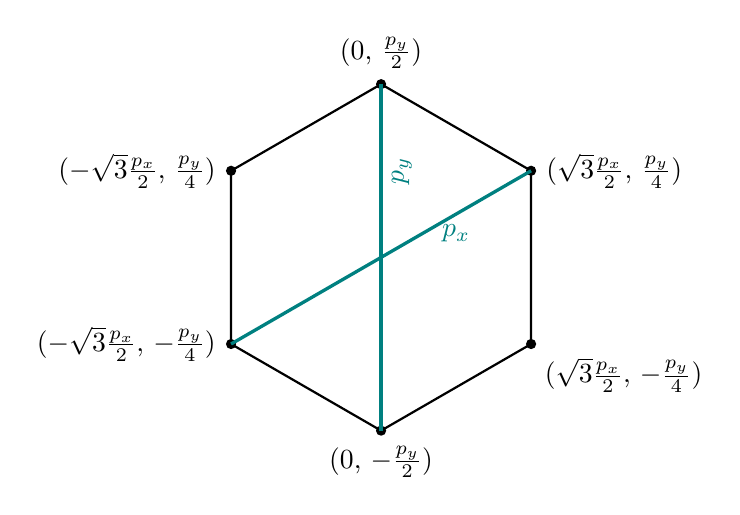
\begin{tikzpicture}[thick]
     \newdimen\R
     \R=2.2cm
     \draw (330:\R) \foreach \x in {30,90,...,330} {  -- (\x:\R) };
     \foreach \x/\l/\p in
       { 30/{($\sqrt{3} \frac{p_x}{2}$, $\frac{p_y}{4}$)}/right,
        90/{($0$, $\frac{p_y}{2}$)}/above,
        150/{($-\sqrt{3} \frac{p_x}{2}$, $\frac{p_y}{4}$)}/left,
        210/{($-\sqrt{3} \frac{p_x}{2}$, $-\frac{p_y}{4}$)}/left,
        270/{($0$, $-\frac{p_y}{2}$)}/below,
        330/{($\sqrt{3} \frac{p_x}{2}$, $-\frac{p_y}{4}$)}/below right
       }
       \node[inner sep=1pt,circle,draw,fill,label={\p:\l}] at (\x:\R) {};

       \draw[very thick, teal] (30:\R) -- (210:\R) node[near start, below] {$p_x$};

       \draw[very thick, teal] (270:\R) -- (90:\R) node[sloped, near end, below] {$p_y$};

\end{tikzpicture}

        \caption{Hexagon in \emph{pointy} orientation}
        \label{fig:hexagon:pointy}
    \end{subfigure}%
    \begin{subfigure}[b]{0.5\textwidth}
        \centering
        \tikzset{%
  >=latex
}
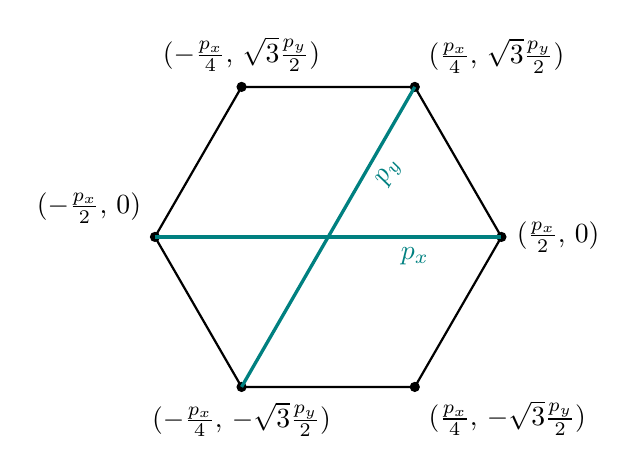
\begin{tikzpicture}[thick]
     \newdimen\R
     \R=2.2cm
     \draw (0:\R) \foreach \x in {60,120,...,360} {  -- (\x:\R) };
     \foreach \x/\l/\p in
       { 60/{($\frac{p_x}{4}$, $\sqrt{3} \frac{p_y}{2}$)}/above right,
        120/{($-\frac{p_x}{4}$, $\sqrt{3} \frac{p_y}{2}$)}/above,
        180/{($-\frac{p_x}{2}$, $0$)}/above left,
        240/{($-\frac{p_x}{4}$, $-\sqrt{3} \frac{p_y}{2}$)}/below,
        300/{($\frac{p_x}{4}$, $-\sqrt{3} \frac{p_y}{2}$)}/below right,
        360/{($\frac{p_x}{2}$, $0$)}/right
       }
       \node[inner sep=1pt,circle,draw,fill,label={\p:\l}] at (\x:\R) {};

       \draw[very thick, teal] (360:\R) -- (180:\R) node[near start, below] {$p_x$};

       \draw[very thick, teal] (240:\R) -- (60:\R) node[sloped, near end, below] {$p_y$};

\end{tikzpicture}

        \caption{Hexagon in \emph{flat} orientation}
        \label{fig:hexagon:flat}
    \end{subfigure}%
    \caption{Definition of the pitches $p_x$ and $p_y$, and corner positions for the pointy (\subref{fig:hexagon:pointy}) and flat (\subref{fig:hexagon:flat}) hexagon orientation in Cartesian coordinates. The pitches align with the axes of the axial coordinate system of the hexagonal grid.}
    \label{fig:hexagon}
\end{figure}

Hexagonal pixel grids in \apsq use an axial coordinate system to describe the relative positions and indices of hexagons on the grid, following largely the definitions provided in~\cite{hexagons}.
Similar to the Cartesian coordinate system used for regular pixel layouts, the origin is the lower-left corner of the sensor, with the hexagon indices $(0,0)$.
Owing to the orientation of the grid axes, negative can occur in the top-left region of the sensor.

Two orientations of hexagons are supported, subsequently referred to as \emph{pointy} with sides parallel to the $y$ axis of the Cartesian coordinate system and corners at the top and bottom, and \emph{flat} with sides parallel to the Cartesian $x$ axis and corners to the left and right.
The pitches $p_x$ and $p_y$ of the hexagon align with the axial coordinate system and are rotated differently with respect to the Cartesian system between the two variants.
The orientation of the pitches as well as the resulting corner positions in Cartesian coordinates are shown in Figure~\ref{fig:hexagon}.

The additional parameters for the \textbf{hexagonal} model are as follows:
\begin{itemize}
\item \parameter{pixel_type}: The shape/orientation of the hexagonal pixels within the grid, either \parameter{hexagon_pointy} or \parameter{hexagon_flat}.
\end{itemize}

\begin{figure}[tbp]
    \centering
    \begin{subfigure}[b]{0.5\textwidth}
        \centering
        \tikzset{%
  >=latex
}
\begin{tikzpicture}[y=7.5mm,x=4.34mm,thick]
  \tikzset{
    box/.style={
      regular polygon,
      regular polygon sides=6,
      minimum size=10mm,
      inner sep=0mm,
      outer sep=0mm,
      rotate=30,
    draw
    }
  }

\foreach \i in {0,...,7}
    \foreach \j in {0,...,1} {
            \node[box] at (2*\i-1,2*\j) {};
            \node[box] at (2*\i,2*\j+1) {};
        }
\end{tikzpicture}

        \caption{\si{8x4} grid with \emph{pointy} hexagons}
        \label{fig:hexagongrid:pointy}
    \end{subfigure}%
    \begin{subfigure}[b]{0.5\textwidth}
        \centering
        \tikzset{%
  >=latex
}
\begin{tikzpicture}[x=7.5mm,y=4.34mm,thick]
  \tikzset{
    box/.style={
      regular polygon,
      regular polygon sides=6,
      minimum size=10mm,
      inner sep=0mm,
      outer sep=0mm,
      rotate=0,
    draw
    }
  }

\foreach \i in {0,...,3}
    \foreach \j in {0,...,3} {
            \node[box] at (2*\i,2*\j) {};
            \node[box] at (2*\i+1,2*\j+1) {};
        }
\end{tikzpicture}

        \caption{\si{8x4} grid with \emph{flat} hexagons}
        \label{fig:hexagongrid:flat}
    \end{subfigure}%
    \caption{Grid layouts for \emph{pointy} (\subref{fig:hexagongrid:pointy}) and \emph{flat} (\subref{fig:hexagongrid:flat}) hexagons with a size of \si{8x4} pixels.}
    \label{fig:hexagongrid}
\end{figure}

The number of pixels in a hexagonal grid are counted along the Cartesian axes, taking the offset pixels into account.
For example, an \si{8x4} grid comprises \num{32} pixels both for \emph{pointy} and \emph{flat} hexagon orientation, but results in different overall grid dimensions as demonstrated in Figure~\ref{fig:hexagongrid}.

\nlparagraph{Support Layers}
\label{sec:support_layers}
In addition to the active layer, multiple layers of support material can be added to the detector description.
It is possible to place support layers at arbitrary positions relative to the sensor, while the default position is behind the readout chip (or inactive silicon layer).
The defined support materials will always be positioned relative to the corresponding detector.
The support material can be chosen either from a set of predefined materials, including PCB and Kapton, or any material available via the Geant4 material database.

Every support layer should be defined in its own section headed with the name \texttt{[support]}.
By default, no support layers are added.
Support layers allow for the following parameters.
\begin{itemize}
\item \parameter{size}: Size of the support in 2D (the thickness is given separately below).
This parameter is required for all support layers.
\item \parameter{thickness}: Thickness of the support layers.
This parameter is required for all support layers.
\item \parameter{location}: Location of the support layer.
Either \textit{sensor} to attach it to the sensor (opposite to the readout chip/inactive silicon layer), \textit{chip} to add the support layer behind the chip/inactive layer or \textit{absolute} to specify the offset in the z-direction manually.
Defaults to \textit{chip} if not specified.
If the parameter is equal to \textit{sensor} or \textit{chip}, the support layers are stacked in the respective direction when multiple layers of support are specified.
\item \parameter{offset}: If the parameter \parameter{location} is equal to \textit{sensor} or \textit{chip}, an optional 2D offset can be specified using this parameter, the offset in the z-direction is then automatically determined.
These support layers are by default centered around the middle of the pixel matrix (the rotation center of the model).
If the \texttt{location} is set to \textit{absolute}, the offset is a required parameter and should be provided as a 3D vector with respect to the center of the model (thus the center of the active sensor).
Care should be taken to ensure that these support layers and the rest of the model do not overlap.
\item \parameter{hole_size}: Adds an optional cut-out hole to the support with the 2D size provided.
The hole always cuts through the full support thickness.
No hole will be added if this parameter is not present.
\item \parameter{hole_type}: Type of hole to be punched into the support layer. Currently supported are \textit{rectangle} and \textit{cylinder}. Defaults to \textit{rectangle}.
\item \parameter{hole_offset}: If present, the hole is by default placed at the center of the support layer.
A 2D offset with respect to its default position can be specified using this parameter.
\item \texttt{material}: Material of the support. \apsq does not provide a set of materials to choose from; it is up to the modules using this parameter to implement the materials such that they can use it.
Chapter~\ref{ch:modules} provides details about the materials supported by the geometry builder module (\parameter{GeometryBuilderGeant4}).
\todo{This should be standardized...}
\end{itemize}

\nlparagraph{Accessing specific detector models within the framework}
Some modules are written to act on only a particular type of detector model.
In order to ensure that a specific detector model has been used, the model should be downcast: the downcast returns a null pointer if the class is not of the appropriate type.
An example for fetching a \texttt{HybridPixelDetectorModel} would thus be:
\begin{minted}[frame=single,framesep=3pt,breaklines=true,tabsize=2,linenos]{c++}
// "detector" is a pointer to a Detector object
auto model = detector->getModel();
auto hybrid_model = std::dynamic_pointer_cast<HybridPixelDetectorModel>(model);
if(hybrid_model != nullptr) {
    // The model of this Detector is a HybridPixelDetectorModel
}
\end{minted}

\nlparagraph{Specializing detector models}
A detector model contains default values for all parameters.
Some parameters like the sensor thickness can however vary between different detectors of the same model.
To allow for easy adjustment of these parameters, models can be specialized in the detector configuration file introduced in~\ref{sec:detector_config}.
All model parameters, except the type parameter and the support layers, can be changed by adding a parameter with the exact same key and the updated value to the detector configuration.
The framework will then automatically create a copy of this model with the requested change.

\begin{warning}
Before re-implementing models, it should be checked if the desired change can be achieved using the detector model specialization. For most cases this provides a quick and flexible way to adapt detectors to different needs and setups (for example, detectors with different sensor thicknesses).
\end{warning}

\nlparagraph{Search order for models}
To support different detector models and storage locations, the framework searches different paths for model files in the following order:
\begin{enumerate}
\item If defined, the paths provided in the global \parameter{model_paths} parameter are searched first.
Files are read and parsed directly.
If the path is a directory, all files in the directory are added (without recursing into subdirectories).
\item The location where the models are installed to (refer to the description of the \parameter{MODEL_DIRECTORY} variable in Section~\ref{sec:cmake_config}).
\item The standard data paths on the system as given by the environmental variable \parameter{$XDG_DATA_DIRS} with ``\project/models'' appended.
The \parameter{$XDG_DATA_DIRS} variable defaults to \textit{/usr/local/share/} (thus effectively \textit{/usr/local/share/\project/models}) followed by \textit{/usr/share/} (effectively \textit{/usr/share/\project/models}).
\end{enumerate}

\section{Passing Objects using Messages}
\label{sec:objects_messages}
Communication between modules is performed by the exchange of messages.
Messages are templated instantiations of the \parameter{Message} class carrying a vector of objects.
The list of objects available in the \apsq objects library are discussed in Chapter~\ref{ch:objects}.
The messaging system has a dispatching mechanism to send messages and a receiving part that fetches incoming messages.
Messages are always received by modules in the order they have been dispatched by preceding modules.

The dispatching module can specify an optional name for the messages, but modules should normally not specify this name directly.
If the name is not given (or equal to \texttt{-}) the \parameter{output} parameter of the module is used to determine the name of the message, defaulting to an empty string.
Dispatching messages to their receivers is then performed following these rules:
\begin{enumerate}
    \item The receiving module will \underline{only} receive a message if it has the exact same type as the message dispatched (thus carrying the same objects).
    If the receiver is however listening to the \parameter{BaseMessage} type which does not specify the type of objects it is carrying, it will instead receive all dispatched messages.
    \item The receiving module will \underline{only} receive messages with the exact name it is listening for.
    The module uses the \parameter{input} parameter to determine which message names it should listen for; if the \parameter{input} parameter is equal to \texttt{*} the module will listen to all messages.
    Each module by default listens to messages with no name specified (thus receiving the messages of dispatching modules without output name specified).
    \item If the receiving module is a detector module, it will \underline{only} receive messages bound to that specific detector \underline{or} messages that are not bound to any detector.
\end{enumerate}

An example of how to dispatch a message containing an array of \parameter{Object} types bound to a detector named \texttt{dut} is provided below.
As usual, the message is dispatched at the end of the \parameter{run()} function of the module.
\begin{minted}[frame=single,framesep=3pt,breaklines=true,tabsize=2,linenos]{c++}
void run(Event* event) {
    std::vector<Object> data;
    // ..fill the data vector with objects ...

    // The message is dispatched only for the module's detector, stored in "detector_"
    auto message = std::make_shared<Message<Object>>(data, detector_);

    // Send the message using the Messenger object for the given event
    messenger->dispatchMessage(this, message, event);
}
\end{minted}

\subsection{Methods to process messages}
The message system has multiple methods to process received messages.
The first two are the most common methods and the third should be avoided in almost every instance.
\begin{enumerate}
\item Bind a \textbf{single message} to the input of this module.
This should usually be the preferred method, where a module expects only a single message to arrive per event containing the list of all relevant objects.
The following example binds to a message containing an array of objects and is placed in the constructor of a detector-type \parameter{TestModule}:
\begin{minted}[frame=single,framesep=3pt,breaklines=true,tabsize=2,linenos]{c++}
TestModule(Configuration&, Messenger* messenger, std::shared_ptr<Detector>) {
    // Subscribe to a single message, with no special messenger flags
    messenger->bindSingle<ExampleMessage>(this, MsgFlags::NONE);
}
\end{minted}
\item Bind a \textbf{set of messages} to the input of the module.
This method should be used if the module can (and expects to) receive the same message multiple times (possibly because it wants to receive the same type of message for all detectors).
An example to bind multiple messages containing an array of objects in the constructor of a unique-type \parameter{TestModule} would be:
\begin{minted}[frame=single,framesep=3pt,breaklines=true,tabsize=2,linenos]{c++}
TestModule(Configuration&, Messenger* messenger, GeometryManager* geo_manager) {
    // Subscribe to multiple messages, with no special messenger flags
    messenger->bindMulti<Message<Object>>(this, MsgFlags::NONE);
}
\end{minted}
\item Listen to a particular message type and execute a \textbf{filter function} as soon as an object is received.
This can be used for more advanced strategies of retrieving messages, but the other methods should be preferred whenever possible.
The listening module should \underline{not} do any heavy work in the filtering function as this is supposed to take place in the module \command{run} method instead.
The filter function should return a boolean, indicating whether the message is wanted or not.
Using a filter function can lead to unexpected behavior because the function is executed during the run method of the dispatching module.
This means that logging is performed at the level of the dispatching module and that the filter method can be accessed from multiple threads if the dispatching module is parallelized.
Listening to a message containing an array of objects in a detector-specific \parameter{TestModule} could be performed as follows:
\begin{minted}[frame=single,framesep=3pt,breaklines=true,tabsize=2,linenos]{c++}
TestModule(Configuration&, Messenger* messenger, std::shared_ptr<Detector>) {
    messenger->registerFilter(this,
                              /* Pointer to the filter method */
                              &TestModule::filter,
                              /* No special message flags */
                              MsgFlags::NONE);
}
bool filter(std::shared_ptr<Message<Object>> message) const {
    // Decide if the message is wanted ...
}
\end{minted}
\end{enumerate}

\subsection{Message flags}
\label{sec:messageflags}
Flags can be added to the bind and listening methods which enable a particular behavior of the framework.
\begin{itemize}
    \item \textbf{REQUIRED}: Specifies that this message is required during the event processing.
    If this particular message is not received before it is time to execute the module's run function, the execution of the method is automatically skipped by the framework for the current event.
    This can be used to ignore modules which cannot perform any action without received messages, for example charge carrier propagation without any deposited charge carriers.
    \item \parameter{ALLOW_OVERWRITE}: By default an exception is automatically raised if a single bound message is overwritten (thus receiving it multiple times instead of once).
    This flag prevents this behavior.
    It can only be used for variables bound to a single message.
    \item \parameter{IGNORE_NAME}: If this flag is specified, the name of the dispatched message is not considered.
    Thus, the \parameter{input} parameter is ignored and forced to the value \texttt{*}.
\end{itemize}

\subsection{Persistency}
\label{ch:objects_persistency}
As objects may contain information relating to other objects, in particular for storing their corresponding Monte Carlo history (see Section~\ref{sec:objhistory}), objects are by default persistent until the end of each event. All messages are stored as shared pointers and are released at the end of each event. If no other copies of the shared message pointer are created, then these will be subsequently deleted, including the objects stored therein. Where a module requires access to data from a previous event (such as to simulate the effects of pile-up etc.), local copies of the data objects must be created. Note that at the point of creating copies the corresponding history will be lost.


\section{Redirect Module Inputs and Outputs}
\label{sec:redirect_module_input_outputs}
In the \apsq framework, modules exchange messages typically based on their input and output message types and the detector type.
It is, however, possible to specify a name for the incoming and outgoing messages for every module in the simulation.
Modules will then only receive messages dispatched with the name provided and send named messages to other modules listening for messages with that specific name.
This enables running the same module several times for the same detector, e.g.\ to test different parameter settings.

The message output name of a module can be changed by setting the \parameter{output} parameter of the module to a unique value.
The output of this module is then not sent to modules without a configured input, because by default modules listens only to data without a name.
The \parameter{input} parameter of a particular receiving module should therefore be set to match the value of the \parameter{output} parameter.
In addition, it is permitted to set the \parameter{input} parameter to the special value \texttt{*} to indicate that the module should listen to all messages irrespective of their name.

An example of a configuration with two different settings for the digitization module is shown below:
\begin{minted}[frame=single,framesep=3pt,breaklines=true,tabsize=2,linenos]{ini}
# Digitize the propagated charges with low noise levels
[DefaultDigitizer]
# Specify an output identifier
output = "low_noise"
# Low amount of noise added by the electronics
electronics_noise = 100e
# Default values are used for the other parameters

# Digitize the propagated charges with high noise levels
[DefaultDigitizer]
# Specify an output identifier
output = "high_noise"
# High amount of noise added by the electronics
electronics_noise = 500e
# Default values are used for the other parameters

# Save histogram for 'low_noise' digitized charges
[DetectorHistogrammer]
# Specify input identifier
input = "low_noise"

# Save histogram for 'high_noise' digitized charges
[DetectorHistogrammer]
# Specify input identifier
input = "high_noise"
\end{minted}

\todo{Maybe we need an option to split the modules}

\section{Logging and other Utilities}
\label{sec:logging_utilities}
The \apsq framework provides a set of utilities which improve the usability of the framework and extend the functionality provided by the \CPP Standard Template Library (STL).
The former includes a flexible and easy-to-use logging system, introduced in Section~\ref{sec:logger} and an easy-to-use framework for units that supports converting arbitrary combinations of units to common base units which can  be used transparently throughout the framework, and which will be discussed in more detail in Section~\ref{sec:unit_system}.
The latter comprise tools which provide functionality the {\CPP}17 standard does not contain.
These utilities are used internally in the framework and are only shortly discussed in Section~\ref{sec:filesystem} (file system support) and Section~\ref{sec:string_utilities} (string utilities).

\subsection{Logging system}
\label{sec:logger}
The logging system is built to handle input/output in the same way as \texttt{std::cin} and \texttt{std::cout} do.
This approach is both very flexible and easy to read.
The system is globally configured, thus only one logger instance exists.
The following commands are available for sending messages to the logging system at a level of \parameter{LEVEL}:

\begin{description}
    \item[\command{LOG(LEVEL)}] Send a message with severity level \parameter{LEVEL} to the logging system.
    \begin{minted}[frame=single,framesep=3pt,breaklines=true,tabsize=2,linenos]{c++}
    LOG(LEVEL) << "this is an example message with an integer and a double " << 1 << 2.0;
    \end{minted}
    A new line and carriage return is added at the end of every log message.
    Multi-line log messages can be used by adding new line commands to the stream. The logging system will automatically align every new line under the previous message and will leave the header space empty on new lines.
    \item[\command{LOG_ONCE(LEVEL)}] Same as \command{LOG}, but will only log this message once over the full run, even if the logging function is called multiple times.
    \begin{minted}[frame=single,framesep=3pt,breaklines=true,tabsize=2,linenos]{c++}
    LOG_ONCE(INFO) << "This message will appear once only, even if present in every event...";
    \end{minted}
    This can be used to log warnings or messages e.g.\ from the \command{run()} function of a module without flooding the log output with the same message for every event.
    The message is preceded by the information that further messages will be suppressed.
    \item[\command{LOG_N(LEVEL, NUMBER)}] Same as \command{LOG_ONCE} but allows to specify the number of times the message will be logged via the additional parameter \parameter{NUMBER}.
    \begin{minted}[frame=single,framesep=3pt,breaklines=true,tabsize=2,linenos]{c++}
    LOG_N(INFO, 10) << "This message will appear maximally 10 times throughout the run.";
    \end{minted}
    The last message is preceded by the information that further messages will be suppressed.
    \item[\command{LOG_PROGRESS(LEVEL, IDENTIFIER)}] This function allows to update the message to be updated on the same line for simple progressbar-like functionality.
    \begin{minted}[frame=single,framesep=3pt,breaklines=true,tabsize=2,linenos]{c++}
    LOG_PROGRESS(STATUS, "EVENT_LOOP") << "Running event " << n << " of " << number_of_events;
    \end{minted}
    Here, the \parameter{IDENTIFIER} is a unique string identifying this output stream in order not to mix different progress reports.
\end{description}

If the output is a terminal screen the logging output will be coloured to make it easier to identify warnings and error messages.
This is disabled automatically for all non-terminal outputs.

More details about the logging levels and formats can be found in Section~\ref{sec:logging_verbosity}.

\subsection{Unit system}
\label{sec:unit_system}
Correctly handling units and conversions is of paramount importance.
Having a separate \CPP type for every unit would however be too cumbersome for a lot of operations, therefore units are stored in standard \CPP floating point types in a default unit which all code in the framework should use for calculations.
In configuration files, as well as for logging, it is however very useful to provide quantities in different units.

The unit system allows adding, retrieving, converting and displaying units.
It is a global system transparently used throughout the framework.
Examples of using the unit system are given below:
\begin{minted}[frame=single,framesep=3pt,breaklines=true,tabsize=2,linenos]{c++}
// Define the standard length unit and an auxiliary unit
Units::add("mm", 1);
Units::add("m", 1e3);
// Define the standard time unit
Units::add("ns", 1);
// Get the units given in m/ns in the defined framework unit (mm/ns)
Units::get(1, "m/ns");
// Get the framework unit (mm/ns) in m/ns
Units::convert(1, "m/ns");
// Return the unit in the best type (lowest number larger than one) as string.
// The input is in default units 2000mm/ns and the 'best' output is 2m/ns (string)
Units::display(2e3, {"mm/ns", "m/ns"});
\end{minted}

A description of the use of units in config files within \apsq was presented in Section~\ref{sec:config_values}.

\subsection{Internal utilities}
\label{sec:string_utilities}
STL only provides string conversions for standard types using \texttt{std::stringstream} and \texttt{std::to\_string}, which do not allow parsing strings encapsulated in pairs of double quote (\texttt{"}) characters nor integrating different units.
Furthermore it does not provide wide flexibility to add custom conversions for other external types in either way.

The \apsq \texttt{to\_string} and \texttt{from\_string} methods provided by its \textbf{string utilities} do allow for these flexible conversions, and are extensively used in the configuration system.
Conversions of numeric types with a unit attached are automatically resolved using the unit system discussed above.
The string utilities also include trim and split strings functions missing in the STL.

Furthermore, the \apsq tool system contains extensions to allow automatic conversions for ROOT and Geant4 types as explained in Section~\ref{sec:root_and_geant4_utilities}.


\section{Error Reporting and Exceptions}
\label{sec:error_reporting_exceptions}
\apsq generally follows the principle of throwing exceptions in all cases where something is definitely wrong.
Exceptions are also thrown to signal errors in the user configuration.
It does not attempt to circumvent problems or correct configuration mistakes, and the use of error return codes is to be discouraged.
The asset of this method is that errors cannot easily be ignored and the code is more predictable in general.

For warnings and information messages, the logging system should be used extensively.
This helps both in following the progress of the simulation and in debugging problems.
Care should however be taken to limit the amount of messages in levels higher than \texttt{DEBUG} or \texttt{TRACE}.
More details about the logging levels and their usage can be found in Section~\ref{sec:logging_verbosity}.

The base exceptions in \apsq are available via the utilities.
The most important exception base classes are the following:
\begin{itemize}
\item \parameter{ConfigurationError}: All errors related to incorrect user configuration.
This could indicate a non-existing configuration file, a missing key or an invalid parameter value.
\item \parameter{RuntimeError}: All other errors arising at run-time.
Could be related to incorrect configuration if messages are not correctly passed or non-existing detectors are specified.
Could also be raised if errors arise while loading a library or executing a module.
\item \parameter{LogicError}: Problems related to modules which do not properly follow the specifications, for example if a detector module fails to pass the detector to the constructor.
These methods should never be raised for correctly implemented modules and should therefore not be of any concern for the end users.
Reporting this type of error can help developers during the development of new modules.
\end{itemize}

There are only four exceptions that are supposed to be used in specific modules, outside of the core framework.
These exceptions should be used to indicate errors that modules cannot handle themselves:
\begin{itemize}
\item \parameter{InvalidValueError}: Derived from configuration exceptions.
Signals any problem with the value of a configuration parameter not related to parsing or conversion to the required type.
Can for example be used for parameters where the possible valid values are limited, like the set of logging levels, or for paths that do not exist.
An example is shown below:
\begin{minted}[frame=single,framesep=3pt,breaklines=true,tabsize=2,linenos]{c++}
void run(Event* event) {
    // Fetch a key from the configuration
    std::string value = config.get("key");

    // Check if it is a 'valid' value
    if(value != 'A' && value != "B") {
        // Raise an error if it the value is not valid
        //   provide the configuration object, key and an explanation
        throw InvalidValueError(config, "key", "A and B are the only allowed values");
    }
}
\end{minted}
\item \parameter{InvalidCombinationError}: Derived from configuration exceptions.
Signals any problem with a combination of configuration parameters used.
This could be used if several optional but mutually exclusive parameters are present in a module, and it should be ensured that only one is specified at the time.
The exceptions accepts the list of keys as initializer list.
An example is shown below:
\begin{minted}[frame=single,framesep=3pt,breaklines=true,tabsize=2,linenos]{c++}
void run(Event* event) {
    // Check if we have mutually exclusive options defined:
    if(config.count({"exclusive_opt_a", "exclusive_opt_b"}) > 1) {
        // Raise an error if the combination of keys is not valid
        //   provide the configuration object, keys and an explanation
        throw InvalidCombinationError(config, {"exclusive_opt_a", "exclusive_opt_b"}, "Options A and B are mutually exclusive, specify only one.");
    }
}
\end{minted}

\item \parameter{ModuleError}: Derived from module exceptions.
Should be used to indicate any runtime error in a module not directly caused by an invalid configuration value, for example that it is not possible to write an output file.
A reason should be given to indicate what the source of problem is.
\todo{The module class should be passed as well, so the module name can be displayed in the error message}
\item \parameter{EndOfRunException}: Derived from module exceptions.
Should be used to request the end of event processing in the current run, e.g. if a module reading in data from a file reached the end of its input data.
\end{itemize}

\todo{add more info about error reporting style?}

\section{Multithreading}
\label{sec:multithreading_approach}
\apsq supports multithreading by running events in parallel.
The module manager creates a thread pool with the configured number of workers or determines them from system parameters if not specified.
Each event is represented by an instance of the \texttt{Event} class which encapsulates the data used during this event.
The configured number of events are then submitted to the thread pool and executed by the thread pool's workers.

The thread pool features two independent queues.
A FIFO-like unsorted queue for events to be processed, and a second, priority-ordered queue for buffered events.
The former is constantly filled with new events to be processed by the main thread, while the latter is used to temporarily buffer events which wait to be picked up in the correct sequence by a \texttt{SequentialModule}.

By default modules are assumed to not operate in a thread-safe way and therefore cannot participate in multithreaded processing of events.
Therefore each module must explicitly enable multithreading in its constructor in order to signal its multithreading capabilities to \apsq.
To support multithreading, the module \texttt{run()} method should be re-entrant and any shared member variables should be protected.
If multithreading is enabled in the run configuration, the module manager will check if all the loaded modules support multithreading.
In case one or more modules do not support multithreading, a warning is printed and the feature is disabled. Modules can inform themselves about the decision via the \texttt{multithreadingEnabled()} method.

\subsection{Seed Distribution}
A stable seed distribution to modules and core components of \apsq is guaranteed in order to be able to provide reproducibility of simulation results from the same inputs even when the number of workers is different.
Each event is seeded upon its creation by the main thread from a central event seed generator, in increasing sequence of event numbers. The event provides access to a random engine that can be used by each module in the \texttt{run()} method.

To avoid the memory overhead of maintaining random engine objects equal to the number of events, the storage of the engines is made static and thread-local, and is only provided to the event for temporary usage.
This way ensures that the framework maintains the minimum number of such heavy objects equal to the number of workers used.
When a worker starts to execute a new event, it seeds its local random engine first and passes it to the event object.

\subsection{Using Messenger in Parallel}
The \texttt{Messenger} handles communication in different events concurrently. It supports dispatching and fetching messages via the \texttt{LocalMessenger}.
Each event has its own local messenger which stores all messages that was produced in this event.
The \texttt{Messenger} owns the global message subscription information and internally forwards the module's requests to dispatch or fetch messages to the local messenger of the event in a thread-safe manner.

\subsection{Running Events in order using SequentialModule}
The \texttt{SequentialModule} class is made available for modules that require processing of events in the correct order without disabling multithreading.
Inheriting from this class will allow the module to transparently check if the given event is in the correct sequence and decide whether to execute it immediately or to request buffering in the prioritized buffer queue if the thread pool if it is out of order.

Using the \texttt{SequentialModule} is suitable for I/O modules which read or write to the file system and do not allow random read or write access to events.
This enables output modules to produce the exact same output file for the same simulation inputs without sacrificing the benefits of using multithreading for other modules.

Since random number generators are thread-local and shared between events processed on the same thread, their state is stored internally when being written into the buffer and restored before processing.
This ensures that the sequence of pseudo-random numbers is exactly the same regardless of whether the event was buffered or directly processed.

\subsection{Geant4 Modules}
The usage of the \emph{Geant4} library in \apsq has some constraints because the \emph{Geant4} multithreaded run manager expects to handle parallelization internally which violates the \apsq design.
Furthermore, \emph{Geant4} does not guarantee results reproducibility between its multithreaded and sequential run managers.
Modules that would like to use the \emph{Geant4} library shall not use the run managers provided by \emph{Geant4}.
Instead, they must use the custom run managers provided by \apsq as described in Section~\ref{sec:geant4_interface}.
